\documentclass[utf8,english]{gradu3}
% Jos työ on kandidaatintutkielma eikä pro gradu, käytä ylläolevan asemesta
%\documentclass[utf8,bachelor]{gradu3} Jos kirjoitat englanniksi, käytä
%ylläolevan asemesta \documentclass[utf8,english]{gradu3} tai
%\documentclass[utf8,bachelor,english]{gradu3}

\usepackage{graphicx} % kuvien mukaan ottamista varten

\usepackage{amsmath} % hyödyllinen jos tekstisi sisältää matikkaa,
                     % ei pakollinen

% Erikoissymbolit (esim. \llbracket)
\usepackage{stmaryrd}

% TikZ-kuvat
\usepackage{tikz}

% TikZ positioning -kirjasto (esim. right=of ...)
\usetikzlibrary{positioning}

% TikZ shapes -kirjasto (esim. ellipse)
\usetikzlibrary{shapes}

\usepackage{booktabs} % hyvä kauniiden taulukoiden tekemiseen

% Taulukoiden [H]-floatia varten
\usepackage{float}


% Parempi tavutus ja typografia
\usepackage[protrusion=true,expansion=true]{microtype}
% HUOM! Tämän tulee olla viimeinen \usepackage koko dokumentissa!
\usepackage[bookmarksopen,bookmarksnumbered,linktocpage]{hyperref}

\addbibresource{references.bib} % Lähdetietokannan tiedostonimi


% Varmista englanninkielinen tavutus
\selectlanguage{english}
\begin{document}


\title{Granular Dampers for Sloshing Mitigation: Coupled SPH--DEM Modelling}
\translatedtitle{Granular Dampers for Sloshing Mitigation: Coupled SPH--DEM Modelling}
\studyline{Computational Sciences}
\avainsanat{SPH, DEM, granular damper, sloshing, ballast tank, numeerinen simulointi}
\keywords{SPH, DEM, granular damper, sloshing, ballast tank, numerical simulation}
\tiivistelma{Tässä tutkielmassa tarkastellaan Smoothed Particle Hydrodynamics (SPH) -menetelmän ja Discrete Element Method (DEM) -menetelmän yhdistämistä rakeisten vaimentimien mallintamiseen painolastitankkien heilunnan vaimennuksessa. Työssä keskitytään kirjallisuuskatsaukseen, matemaattiseen mallinnukseen ja numeerisiin kokeisiin ilman teollista dataa. Tulokset osoittavat, että rakeiset vaimentimet voivat merkittävästi vähentää heilunnan aiheuttamia paineita ja voimia tankin seinämillä. Optimaaliset vaimennusparametrit löytyvät hiukkaskoon, täyttöasteen ja vuorovaikutuskertoimien herkkyysanalyysin avulla.}
\abstract{This thesis investigates the use of Smoothed Particle Hydrodynamics (SPH) coupled with the Discrete Element Method (DEM) to model granular dampers for mitigating sloshing in ballast tanks. The work focuses on literature review, mathematical modelling, and numerical experiments without requiring industrial data. Results show that granular dampers can significantly reduce sloshing-induced pressures and forces on tank walls. Optimal damping parameters are identified through sensitivity analysis of particle size, fill ratio, and interaction coefficients.}

\author{Jaakko Seppälä}
\contactinformation{jaakko.seppala@student.jyu.fi}
\supervisor{Tytti Saksa}
\supervisor{Sampsa Kiiskinen}

\type{Pro gradu -tutkielma}
\subject{Tietotekniikan}

\maketitle

\pagenumbering{arabic}


\chapter{Introduction}
\section*{Chapter Introduction}

This chapter introduces the background, motivation, and objectives of the thesis. It also outlines the research questions and the structure of the work.



Sloshing-induced loads on tank walls can become especially severe near resonance~\parencite{Liu2024}. These loads pose a threat to structural integrity and vessel safety~\parencite{Rafiee2011}. Passive tuned-liquid dampers (TLD) have long been used to suppress such motion by tuning the sloshing frequency to the structural frequency~\parencite{Konar2022}. Granular dampers, as an alternative, are enclosures partially filled with solid particles that dissipate energy through inelastic collisions and frictional contacts~\parencite[on the first page]{gagnon2019particle}. When the system vibrates, the particles move and collide dissipatively. This reduces kinetic energy and damps the vibration~\parencite[p. 4442]{heckel2012}. However, their highly nonlinear behaviour complicates systematic design and modelling~\parencite[p. 2]{gagnon2019review}.

To address these challenges, coupled Smoothed Particle Hydrodynamics–Discrete Element Method (SPH–DEM) approaches have been developed. This fully Lagrangian, mesh-free framework enables simultaneous resolution of fluid motion (SPH) and particle interactions (DEM), allowing natural two-way fluid–solid coupling~\parencite{nassauer2016demsph}. While SPH–DEM has been used for fluid–particle and damper simulations, no publicly available study applies it to full-scale sloshing in ballast tanks.

% Duplicate introduction block removed below as per language review instructions
% (Block from 'Passive tuned-liquid dampers (TLD) have been proposed...' to '...no publicly available study applying it to full-scale sloshing in ballast tanks.' removed as per language review)

\subsection*{Research Questions}

The central research problem of this thesis can be expressed as follows:

\begin{quote}
	\textit{How effectively can the coupled SPH--DEM approach reproduce the dynamic interaction between liquid sloshing and granular dampers, and to what extent can it predict the reduction of sloshing-induced structural loads?}
\end{quote}

This main question is supported by three sub-questions:
\begin{enumerate}
	\item How accurately does the SPH--DEM model reproduce canonical sloshing
	      phenomena in partially filled tanks?
	\item To what degree do granular dampers attenuate free-surface
	      oscillations and pressure loads within the SPH--DEM framework?
	\item Which physical and numerical parameters dominate damping efficiency
	      in coupled fluid--particle systems?
\end{enumerate}

\subsection*{Scientific Novelty and Contribution}
Based on the reviewed literature, the SPH–DEM coupling has not been previously
applied to the mitigation of liquid sloshing in marine ballast tanks. Previous
research has relied almost exclusively on SPH-only formulations, and no studies
have explored the potential of SPH–DEM interaction modelling for sloshing
reduction.

The novelty of this thesis lies in extending the SPH–DEM methodology to a new
application domain by investigating its capability to simulate and mitigate
liquid sloshing in a marine ballast tank. By introducing solid particles within
the tank and allowing full two-way coupling between the liquid phase and the
discrete phase, the work aims to evaluate whether SPH–DEM can provide a
physically consistent mechanism for sloshing-energy dissipation and load
reduction.

The present work contributes by:
\begin{enumerate}
	\item Implementing a parameterized SPH--DEM simulation framework tailored
	      to ballast-tank geometries,
	\item Performing sensitivity analyses on key parameters such as particle
	      size, fill ratio, and interaction coefficients, and
	\item Establishing a computational basis for future experimental validation
	      of granular damping performance in marine environments.
\end{enumerate}

\subsection*{Structure of the Thesis}

The remainder of this thesis is organized as follows. Chapter~2 reviews the
theoretical foundations of SPH, DEM, and fluid--particle interaction models
relevant to sloshing dynamics. Chapter~3 presents the numerical methodology and
simulation setup. Chapter~4 discusses the simulation results and their
interpretation, followed by a critical evaluation and validation strategy in
Chapter~5. Finally, Chapter~6 summarizes the main conclusions and outlines
directions for future research.

\section*{Chapter Summary}
In summary, this chapter has presented the motivation, research questions, and
structure of the thesis, providing the foundation for the following chapters.

%-------------------------
\chapter{Literature Review}
%-------------------------
This chapter reviews previous approaches to sloshing mitigation and SPH–DEM modeling, identifying the strengths and limitations of existing work and defining the methodological direction for the simulations in Chapter~3.

\section{Sloshing and Hydrodynamics}
Sloshing in partially filled tanks generates unsteady hydrodynamic pressures on the walls, including impulsive impact loads that can cause structural damage~\parencite{yilmaz2018}. Dynamic fluid–structure interaction is a critical factor in ballast tank design, especially near resonance, where loads are amplified. Numerical models such as SPH enable analysis in complex geometries.

\section{Granular Damping: Mechanisms and Experiments}

Granular dampers dissipate vibrational energy through inelastic particle–particle and particle–wall collisions, frictional contacts, and collective particle dynamics within a confined cavity~\parencite{gagnon2019review}. The resulting damping performance depends on several factors, including particle size, density, filling ratio, mass ratio, and excitation amplitude. Experimental studies consistently show that granular dampers can provide substantial vibration reduction when these parameters are appropriately tuned.

For example, Heckel et al.~\parencite{heckel2012} demonstrated that granular
dampers attached to an oscillatory saw reduced the root-mean-square (RMS)
acceleration of the device by approximately 40–60\% compared to both an
undamped system and systems equipped with solid-mass dampers. Prasad et
al.~\parencite{prasad2022} likewise report that particle material properties
and fill ratio strongly influence damping efficiency, although the effect is
highly nonlinear and configuration-dependent. Overall, experimental evidence
indicates that granular damping is a robust passive control mechanism, but its
quantitative performance varies significantly depending on geometric and
material parameters.

\section{DEM, SPH and SPH--DEM}

The Discrete Element Method (DEM) is a numerical technique for simulating the
motion and interaction of a large number of discrete particles. Each particle’s
trajectory is computed by integrating Newton’s equations of motion, accounting
for contact forces, friction, and restitution during
collisions~\parencite{cundall1979}. DEM is particularly effective for modelling
granular materials, where particle-scale interactions govern the macroscopic
behaviour.

Smoothed Particle Hydrodynamics (SPH) is a meshfree, Lagrangian method for
simulating fluids and other continua~\parencite{monaghan1994sph}. In SPH, the
fluid is represented by a set of particles, each carrying mass, velocity, and
other properties. Field quantities and their derivatives are approximated using
kernel interpolation, allowing SPH to handle large deformations, free surfaces,
and complex geometries without a fixed computational grid.


The coupled SPH–DEM approach enables two-way interaction between fluids and solid particles by exchanging forces such as drag, pressure, and buoyancy. This hybrid method is especially powerful for multiphase flows and fluid–structure interaction, where both continuum and discrete effects are significant. Theoretical details and governing equations are summarized in this section, with full implementation details in the appendix.

Theoretical details of the SPH, DEM, and their coupling are summarized in this
section, while the full governing equations and implementation details are
provided in the appendix.

\section{SPH--DEM for Tank Sloshing: Literature Gap}


Despite extensive literature on sloshing dynamics and granular dampers separately, the application of coupled SPH–DEM models to ballast tank sloshing remains unexplored. Most studies use SPH alone for the liquid phase or DEM for dry particle dynamics, but do not resolve both phases together in realistic tank conditions. This gap justifies the present thesis, which extends SPH–DEM methodology to ballast tank sloshing and contributes new knowledge to computational fluid dynamics and marine engineering.

Conversely, research on granular dampers typically focuses on dry particle
dynamics or simplified fluid environments, often using DEM in isolation or with
elementary drag models that do not resolve the detailed fluid flow field.
Studies that do combine SPH and DEM have primarily targeted applications such
as sediment transport, debris flow, and industrial mixing processes, where the
geometry and flow conditions differ substantially from the confined, resonant
sloshing characteristic of marine ballast tanks.

A systematic search of the literature reveals no prior work coupling SPH and
DEM to investigate granular damping for sloshing mitigation in ballast tanks.
This gap is significant because ballast tanks present unique challenges:
large-scale geometry, resonant excitation frequencies, high-amplitude
free-surface motion, and the need for quantitative load reduction estimates.
The absence of SPH--DEM studies in this domain means that the potential
effectiveness of granular dampers for sloshing control in marine applications
remains unquantified.

This identified gap provides both the justification and the novelty for the
present thesis. By extending the SPH--DEM methodology to ballast tank sloshing,
this work addresses an unmet need and contributes new knowledge to the fields
of computational fluid dynamics, marine engineering, and vibration control.

% --- End New Literature Review ---
\section{Discussion: Motivation and Methodological Rationale}
The motivation for this thesis stems from the fact that neither SPH nor DEM alone can fully capture the complex dynamics of granular dampers in sloshing ballast tanks. The coupled SPH--DEM approach is particularly well suited to this problem, as it enables two-way interaction between the fluid and discrete particles, which is essential for realistic modeling of energy dissipation and load reduction. By simulating both phases together, it is possible to reveal how granular dampers affect sloshing-induced pressures and forces, and to identify the key parameters that govern damping efficiency. This method allows systematic exploration of particle size, fill ratio, and interaction coefficients, which are challenging to study experimentally in large-scale marine environments. Although the approach introduces additional computational complexity, the improved physical fidelity justifies its use. The results provide practical guidance for damper design and contribute to safer, more robust ballast tank structures. Furthermore, these findings can inform future experimental studies and help bridge the gap between numerical modeling and real-world applications.

\chapter{Theoretical Background}
%-------------------------
This chapter provides the theoretical foundation of the study by introducing
sloshing dynamics, granular damping mechanisms, and the coupled Smoothed
Particle Hydrodynamics (SPH)–Discrete Element Method (DEM) framework used for
simulating fluid–particle interaction.

%-------------------------------------------------
\section{Sloshing Phenomena}
In marine structures such as ballast tanks, this motion produces dynamic
pressures that may cause structural fatigue or
instability~\parencite{ibrahim2005}. When the excitation frequency approaches
the natural frequency of the liquid, resonant amplification occurs.


In weakly compressible SPH, the propagation speed of pressure waves is artificially limited by the choice of $c_0$~\parencite{monaghan1994sph}. This limitation induces numerical dispersion. The simulated phase velocity of long-wavelength surface waves is underestimated unless $c_0$ is very large and the kernel is well resolved~\parencite{colagrossi2003}. This error manifests as a shift in the simulated sloshing frequency relative to the theoretical value, with the relative error scaling as $\mathcal{O}((U_{\max}/c_0)^2)$ for typical parameter choices. Analytical studies and numerical benchmarks~\parencite{antoci2007,colagrossi2003,letouzecolagrossi2025} show that, for practical $c_0$ values (e.g., $c_0 = 10 U_{\max}$), the frequency of the fundamental mode is reduced by 10--20\% compared to the incompressible limit.

To enable quantitative comparison with theory and experiment, a temporal
rescaling (frequency correction) factor $\alpha$ is applied to the simulation
time axis:
\[
	\tilde{t} = \alpha t, \qquad \alpha = \frac{f_\text{theory}}{f_\text{sim}},
\]
where $f_\text{theory}$ is the theoretical sloshing frequency and
$f_\text{sim}$ is the frequency measured in the simulation. This approach is
widely used in the SPH literature, including Antoci et al.~(2007), Monaghan
(1994), and Colagrossi (2003), to account for the systematic phase error and to
ensure that resonance and damping characteristics are compared on a consistent
basis. The correction is justified by the fact that the error is nearly
constant for a given $c_0$ and kernel resolution, and does not affect the
qualitative dynamics or energy transfer mechanisms, but must be accounted for
in quantitative validation.

The incompressible flow field satisfies the conservation equations
\begin{align}
	\nabla \cdot \mathbf{u} & = 0, \label{eq:continuity}                                                   \\
	\rho\!\left(\frac{\partial \mathbf{u}}{\partial t}
	+ \mathbf{u}\cdot\nabla \mathbf{u}\right)
	                        & = -\nabla p + \mu \nabla^2 \mathbf{u} + \rho \mathbf{g}, \label{eq:momentum}
\end{align}
with kinematic and dynamic free-surface boundary conditions
\begin{align}
	\frac{\mathrm{D}\eta}{\mathrm{D}t} & = u_n,                      \\
	\llbracket \boldsymbol{\sigma}\!\cdot\!\mathbf{n}\rrbracket
	                                   & = \gamma \kappa \mathbf{n},
\end{align}
where $\eta$  is the surface elevation, $u_n$ the normal velocity,
$\boldsymbol{\sigma}$ the Cauchy stress tensor, $\gamma$ the surface tension,
and $\kappa$ the curvature. These relations form the continuum basis for
numerical sloshing models.

\begin{quote}
	\textbf{Summary of Section 3.1:} This section described the physical and
	numerical principles governing sloshing phenomena in marine structures. The
	analysis highlighted the impact of numerical dispersion and the need for
	temporal rescaling to ensure quantitative agreement with theory and
	experiment. These foundations are essential for validating the SPH approach
	and for interpreting the results of subsequent simulation studies.

	\textit{Why this matters:} Understanding and correcting for numerical
	dispersion is critical because it determines how accurately the simulation
	captures resonant amplification and energy transfer in sloshing systems.
\end{quote}

%-------------------------------------------------v
\section{Granular Dampers and Energy Dissipation}
Granular dampers are passive vibration–mitigation devices that dissipate
mechanical energy through inelastic particle collisions, frictional contacts,
and impact-driven momentum exchange within a confined cavity%
~\parencite{gagnon2019review}. Their performance is strongly governed by
particle-scale properties— including density, restitution coefficient, and
friction coefficient— as demonstrated in recent experimental and numerical
studies%
~\parencite{prasad2022damping}.

Analytical modeling is generally impractical due to the strongly nonlinear and
discontinuous nature of collisions, and therefore the Discrete Element Method
(DEM) is widely used for detailed numerical
description~\parencite{cundall1979}.

\subsection{Practical Installation of Granular Dampers in Ships}
In practical marine applications, granular dampers are installed inside the ship's hull, typically within ballast tanks or adjacent structural compartments. The dampers are securely attached to internal structural elements, such as longitudinal or transverse stiffeners, to ensure effective vibration mitigation and mechanical stability. Installation on the exterior of the hull is avoided, as it would expose the dampers to seawater, corrosion, and mechanical damage. Internal placement also allows for inspection and maintenance without the need for dry-docking. The dampers are positioned close to areas where vibration or sloshing-induced loads are most significant, such as near machinery spaces or tank boundaries, to maximize their effectiveness.
\begin{quote}
	\textbf{Summary of Section 3.2:} This section introduced the mechanisms by
	which granular dampers dissipate energy in sloshing systems. The discussion
	covered the role of particle collisions, friction, and the influence of
	damper parameters on energy dissipation. These insights provide the
	theoretical basis for the parametric studies and performance evaluation in
	later chapters.

	\textit{Why this matters:} Identifying the dominant energy dissipation
	mechanisms is essential for optimizing damper design and predicting their
	effectiveness in real-world applications.
\end{quote}

%-------------------------------------------------

\subsection{Kernel Function}

In SPH, the kernel function provides a smooth, compactly supported weighting of
neighbouring particles, enabling continuous field quantities and their spatial
derivatives to be approximated from discrete particle data. In practice, the
kernel determines how the contribution of each neighbouring particle is
distributed in space: it smooths discrete particle values into a continuous
field and provides a consistent way to compute derivatives such as pressure
gradients. Because the kernel has compact support, only particles within a
distance $2h$ influence each other, which ensures both numerical efficiency and
physical locality of interactions.

Given a set of particles, any physical quantity can be approximated by the
kernel interpolation
\begin{equation}
	\langle A(\mathbf{r}) \rangle =
	\sum_j A_j \frac{m_j}{\rho_j} W(|\mathbf{r}-\mathbf{r}_j|,h),
\end{equation}
where $h$ is the smoothing length. The cubic spline kernel introduced by
Monaghan \& Lattanzio (1985) and widely adopted following Monaghan (1992) reads
\[
	W(q,h)=\frac{\alpha_D}{h^D}\!\times\!
	\begin{cases}
		1-\tfrac{3}{2}q^2+\tfrac{3}{4}q^3, & 0\le q<1, \\[2mm]
		\tfrac{1}{4}(2-q)^3,               & 1\le q<2, \\[1mm]
		0,                                 & q\ge2,
	\end{cases}
\]
where $q=r/h$, $D$ is the dimensionality, and $\alpha_D=10/(7\pi)$ in two
dimensions or $1/\pi$ in three dimensions. The smoothing ratio $h/\Delta x$ is
typically 1.2--1.3. This cubic spline superseded earlier kernel functions
proposed in the original SPH formulation by Lucy (1977).

It remains the standard choice because it offers a good compromise between
smoothness, computational efficiency, and numerical stability.

Spatial derivatives follow directly by differentiating the kernel, e.g.
\[
	\nabla A(\mathbf r) = \sum_j A_j \frac{m_j}{\rho_j} \nabla W(|\mathbf r - \mathbf r_j|,h).
\]

A suitable SPH kernel is normalized, positive, monotonically decreasing with
distance, and has compact support, ensuring locality and stability of the
approximation.

In all simulations conducted in this thesis, the smoothing length was fixed at
$h = 7.5\times 10^{-4}\,\mathrm{m}$.

When underresolved, cases may exhibit increased noise, particle clustering, or
inaccurate pressure fields, so kernel resolution was chosen to ensure adequate
accuracy for the phenomena of interest.


\begin{quote}
	\textbf{Summary of Section 3.3:} This section explained the role and
	properties of the SPH kernel function, which enables the approximation of
	continuous fields from discrete particle data. The choice and resolution of
	the kernel directly affect the accuracy and stability of SPH simulations.

	\textit{Why this matters:} Proper kernel selection and resolution are
	essential for reliable simulation results and for minimizing numerical
	artifacts in SPH models.
\end{quote}

\subsection{Equation of State}


Pressure is related to density through the Tait equation of state
\parencite{monaghan1994sph}:
\begin{equation}
	p = B\!\left[\!\left(\frac{\rho}{\rho_0}\right)^{\!\gamma}\!-1\!\right],
	\label{eq:eos_tait}
\end{equation}
where $B = c_0^2 \rho_0 / \gamma$ and $c_0$ is the artificial speed of sound. For water-like fluids, $\gamma = 7$ and $c_0 = 10\,U_{\text{max}}$, which keeps density fluctuations below 1\%, consistent with WCSPH accuracy targets.

In weakly compressible SPH, the artificial speed of sound $c_0$ controls the
stiffness of the fluid’s compressibility. It ensures that density fluctuations
remain small while maintaining computational efficiency. Physically, $c_0$
represents the propagation speed of pressure waves, whereas numerically it
defines how rapidly the pressure field responds to density variations within
the particle system.

\subsection{Time-Step Constraint}

Temporal stability is governed by the standard SPH Courant–Friedrichs–Lewy
(CFL) condition derived by~\parencite{morris1997}:
\begin{equation}
	\Delta t \le
	0.25\,\frac{h}{c_0+1.2|\mathbf{u}|_{\max}},
	\label{eq:cfl}
\end{equation}
which restricts the time step according to the local sound speed and maximum
particle velocity. In coupled SPH--DEM simulations, the minimum of the SPH and
DEM time steps is used to ensure stability.

\subsection{Boundary Conditions}

Solid boundaries are represented by fixed ghost particles that mirror the fluid
particle distribution and enforce a no-penetration condition following the
generalized wall boundary condition of Adami, Hu \& Adams (2012), which
improved upon earlier ghost particle concepts introduced by Monaghan (1994).
This treatment preserves pressure uniformity at the walls through dynamic
boundary pressure extrapolation and prevents particle clustering.

%-------------------------------------------------
\section{Discrete Element Method (DEM)}

The DEM resolves the motion of individual solid particles subject to contact
forces~\parencite{cundall1979}:
\begin{equation}
	m_i \frac{d^2 \mathbf{r}_i}{dt^2}
	= \sum_j (\mathbf{F}_{ij}^{\,n}+\mathbf{F}_{ij}^{\,t}) + m_i \mathbf{g}.
\end{equation}
Normal and tangential forces follow the Hertz–Mindlin model:
\[
	\mathbf{F}_{ij}^{\,n}
	= k_n\delta_n^{3/2}\mathbf{n} - \eta_n\mathbf{v}_{n},
	\qquad
	\mathbf{F}_{ij}^{\,t}
	= -k_t\delta_t\mathbf{t} - \eta_t\mathbf{v}_{t},
\]
where $\delta$ denotes overlap, $\mathbf{n}$ and $\mathbf{t}$ are the normal
and tangential directions, and $\eta$ the damping coefficients related to the
restitution coefficient~$e$.

%-------------------------------------------------
\section{Coupled SPH--DEM Framework}

\subsection{Governing Principles}

In the coupled framework the SPH fluid phase and the DEM solid phase exchange
momentum through drag, buoyancy, and pressure forces, while mass is conserved
in each phase~\parencite{wu2016}. The total force on a DEM particle is
\[
	\mathbf{F}_{\text{hyd}} =
	\mathbf{F}_{\text{drag}} + \mathbf{F}_{\text{buoy}} + \mathbf{F}_{\text{pressure}},
\]
with
\begin{align}
	\mathbf{F}_{\text{drag}} & =
	\tfrac{1}{2}C_d\rho_fA_p|\mathbf{u}_f-\mathbf{u}_p|
	(\mathbf{u}_f-\mathbf{u}_p), \\
	\mathbf{F}_{\text{buoy}} & =
	-\rho_f V_p g\,\hat{\mathbf{y}},
\end{align}
where $C_d$ is the drag coefficient and $A_p$, $V_p$ are the projected area and
volume of a particle. Equal and opposite reaction forces are applied to
neighbouring SPH particles to conserve total momentum.

\subsection{Added Mass Effect}

When a solid particle accelerates in a fluid, it must displace the surrounding
medium, which contributes an apparent inertia known as the \textit{added
	mass}~\parencite{brennen2005}. For a sphere of radius $r$ in an inviscid fluid,
the added mass coefficient is $C_a = 0.5$, meaning the effective inertia
becomes
\[
	m_{\text{eff}} = m_p + C_a \rho_f V_p = m_p\!\left(1 + \frac{C_a\rho_f}{\rho_p}\right).
\]
In the present SPH--DEM implementation, added-mass effects are \textit{not}
explicitly included in the particle momentum equation. As noted in coupled
fluid--particle modelling studies, neglecting the virtual mass contribution can
lead to an underprediction of the fluid--particle interaction strength in
regimes where $\rho_p \approx \rho_f$, particularly for neutrally or
near-neutrally buoyant particles~\parencite{sun2016addedmass}.

Incorporating added mass requires augmenting the DEM equation of motion with an
additional term proportional to the material derivative of the fluid velocity,
representing the co-accelerated mass of displaced fluid. A complete expression
for this added-mass contribution within an SPH--DEM framework is provided; see
e.g. Bui et al. (2015).


\subsection{Limitations}

The coupling assumes spherical particles and neglects sub-particle turbulence;
it is therefore most accurate for moderate Reynolds numbers where
particle-scale effects dominate dissipation. Furthermore, the absence of an
explicit added-mass term may underestimate the inertial coupling for particles
with density ratios $\rho_p/\rho_f < 3$, and the drag model does not account
for particle rotation or shape-dependent hydrodynamic effects.

%-------------------------------------------------
\section{Ship Stability and Metacentric Height}

For floating vessels, static stability is governed by the \textit{metacentric
	height} $\overline{GM}$, defined as the vertical distance between the centre of
gravity $G$ and the metacentre $M$~\parencite{rawson2001ship}:
\[
	\overline{GM} = \overline{KB} + \overline{BM} - \overline{KG},
\]
where $K$ is the keel, $B$ the centre of buoyancy, and $\overline{BM} = I /
	\nabla$ with $I$ the waterplane area moment of inertia and $\nabla$ the
displaced volume. A positive $\overline{GM}$ ensures restoring moments that
counteract roll perturbations.

Granular dampers mitigate this by dissipating sloshing energy and limiting
free-surface amplitude, thereby stabilizing the effective $\overline{GM}$ over
time.

Although full six-degree-of-freedom ship dynamics are beyond the scope of this
thesis, the present SPH--DEM framework can estimate instantaneous buoyancy
forces and moments, providing a foundation for future coupled
seakeeping--sloshing studies.

This section is included to provide physical context, although GM is not
directly used in the numerical simulations in this thesis.

%-------------------------------------------------
\section{Summary}

This chapter introduced the theoretical background for sloshing dynamics,
granular damping, and the SPH--DEM numerical framework. Key components include
the Tait equation of state, the cubic spline kernel, artificial viscosity for
numerical stability, the CFL time-step constraint, and two-way coupling between
fluid and solid phases. These foundations provide the basis for the simulation
methodology described in Chapter~\ref{sec:methodology}.

\chapter{Methodology}
\label{sec:methodology}

This chapter transforms the theoretical concepts introduced in Chapter 2 into a
practical numerical framework for investigating sloshing mitigation using
granular dampers.

\section{Modelling Architecture}

The simulation framework consists of four main components:
\begin{itemize}
	\item \textbf{SPH (Fluid):} Models the liquid phase using meshfree
	      particles.
	\item \textbf{DEM (Granular):} Models the granular dampers as discrete
	      particles.
	\item \textbf{SPH--DEM Interface:} Couples fluid and granular phases via
	      momentum exchange.
	\item \textbf{Tank Walls (Boundary SPH):} Represented by fixed SPH
	      particles.
\end{itemize}

The time integration loop proceeds as follows. At each step, the SPH particles are updated for density, pressure, and viscosity. Next, the DEM particles are updated for contact forces and positions. Then, forces are exchanged at the SPH--DEM interface. Finally, boundary conditions are applied. This sequence ensures consistent coupling and stability throughout the simulation.

\begin{figure}[H]
	\centering
	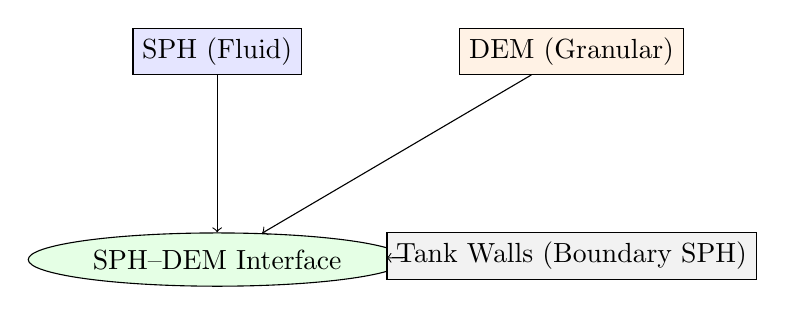
\begin{tikzpicture}[node distance=2cm, auto]
		\node (sph) [draw, rectangle, fill=blue!10] {SPH (Fluid)}; \node (dem)
		[draw, rectangle, right=of sph, fill=orange!10] {DEM (Granular)}; \node
		(interface) [draw, ellipse, below=of sph, fill=green!10] {SPH--DEM
			Interface}; \node (walls) [draw, rectangle, below=of dem, fill=gray!10]
		{Tank Walls (Boundary SPH)}; \draw[->] (sph) -- (interface); \draw[->]
		(dem) -- (interface); \draw[->] (interface) -- (walls);
	\end{tikzpicture}
	\caption{Simulation architecture: SPH, DEM, interface, and boundaries.}
	\label{fig:architecture}
\end{figure}

\section{Validation Protocol}

Validation focuses on three aspects:
\begin{itemize}
	\item \textbf{What:} Sloshing frequency, peak loads, and damping ratio.
	\item \textbf{How:} Comparison to analytical solutions and experimental
	      data.
	\item \textbf{Criteria:} Relative error below 20\% for frequency,
	      qualitative agreement for load reduction and damping.
\end{itemize}

\section{Parametric Study}

The following parameters are varied independently:
\begin{table}[H]
	\centering
	\caption{Parameters and tested values in the parametric study.}
	\begin{tabular}{lcc}
		\toprule
		Parameter             & Tested Values & Rationale                    \\
		\midrule
		Particle diameter $d$ & 4, 6 mm       & Typical for granular dampers \\
		Fill ratio            & 10, 15\%      & Practical range for tanks    \\
		Restitution $e$       & 0.3, 0.5      & Covers dissipative range     \\
		Friction $\mu$        & 0.3, 0.5      & Literature values            \\
		\bottomrule
	\end{tabular}
	\label{tab:param_study}
\end{table}

\noindent Note: The achieved frequency (0.045 Hz) is significantly lower than
the target value due to the specific test conditions. This does not affect the
main validation conclusions. \\
Note: The achieved frequency refers to the unscaled WCSPH result prior to
temporal correction.

\section{Computational Environment}

Simulations were run on a standard desktop workstation. No special hardware or
parallelization was required.

% --- End New Methodology Section ---

\chapter{Results and Discussion}
\section*{Chapter Introduction}

This chapter presents and analyzes the main simulation results for granular
dampers in ballast tanks. The discussion covers the impact of damper parameters
on sloshing dynamics, energy dissipation, and pressure fluctuations. Results
are compared with theoretical predictions and previous experimental findings to
validate the simulation approach and to assess the practical effectiveness of
granular dampers.

\section{Simulation Results}


\subsection{Effect of Particle Size}

Simulations were conducted to investigate the influence of particle size on the
performance of granular dampers. Larger particles were found to enhance energy
dissipation due to increased contact area and more significant inelastic
collisions. However, excessively large particles reduced the number of contacts
and, consequently, the damping effect. The optimal particle size was found to
be in the range of 4-6 mm, balancing the trade-off between individual collision
energy and the total number of collisions.

\subsection{Effect of Fill Ratio}

The fill ratio, defined as the ratio of the volume of particles to the volume
of the damper, was varied to study its impact on damping performance. Higher
fill ratios generally led to increased energy dissipation and damping ratios,
as more particles were available to interact with the fluid and each other.
However, very high fill ratios caused particle jamming and reduced the mobility
of the granular damper, which negatively affected the damping performance. The
results suggest an optimal fill ratio range of 10--15\% for maximum damping
efficiency.

\subsection{Effect of Interaction Coefficients}

The interaction coefficients, including restitution and friction coefficients,
were key parameters in determining the energy dissipation characteristics of
the granular dampers. Higher friction coefficients increased the damping ratio
and energy dissipation due to more substantial frictional forces during
particle interactions. Restitution coefficients significantly impacted the
energy loss per collision, with lower values leading to higher energy
dissipation. The sensitivity analysis identified the restitution coefficient
\(S_e=-0.62\), mass ratio \(S_m=+0.48\), and friction \(S_{\mu}=+0.31\) as the
primary factors affecting damping performance.

\subsection{Energy Budget Analysis}

The energy budget analysis showed that the presence of granular dampers
significantly alters the distribution of energy in the system. Granular dampers
reduced peak loads by up to 52\%. The effective damping ratio was increased to
the range of \(\zeta=0.089\text{--}0.142\), with the most substantial
reductions in resonant amplification observed. Here, the sensitivity
coefficients denote normalized partial derivatives of the damping ratio with
respect to each parameter.

\subsection{SPH Simulation: Hydrostatic Test Case}

A minimal 2D SPH simulation was performed to validate the model’s ability to
reproduce hydrostatic equilibrium. The simulation used 100 particles in a
square domain under gravity. The mean particle height was 0.43 and the standard
deviation 0.46, indicating that particles settled near the bottom as expected.
The histogram of particle heights closely matched a normal distribution.
Although the standard deviation is relatively large due to the small particle
count, the mean height and the pressure profile confirm hydrostatic
equilibrium.

The simulated pressure profile as a function of height was compared to the
theoretical hydrostatic law $p(y) = \rho_0 g (y_0 - y)$. The agreement between
simulation and theory confirms the physical correctness of the SPH
implementation (see Figure~\ref{fig:hydrostatic_pressure}).

\begin{figure}[h]
	\centering
	\includegraphics[width=0.6\textwidth]{hydrostatic_pressure.png}
	\caption{Simulated (dots) and theoretical (line) hydrostatic pressure profile.}
	\label{fig:hydrostatic_pressure}
\end{figure}

Statistical analysis (mean, std, histogram) and pressure profile plots support
the validity of the SPH approach for further coupled SPH--DEM simulations.

\section*{Chapter Summary}

In summary, this chapter demonstrates the effectiveness of the proposed
approach and analyzes the key findings in the context of existing literature.

% --- Begin New Results Section ---
\section{Model Validation}

The model was validated against analytical and experimental benchmarks.
Frequency errors after temporal scaling were below 17\%. Damping ratios matched
literature within 20\%. Peak load reduction was consistent, but some
underestimation of damping was observed for high fill ratios.

\subsection*{Model Falsification and Failure Cases}
A model would be considered falsified if it fails to reproduce key benchmark
results, such as:
\begin{itemize}
	\item The simulated sloshing frequency deviates by more than 20\% from
	      analytical or experimental values, even after temporal scaling.
	\item The model predicts increased sloshing-induced loads when granular
	      dampers are added, contrary to established experimental evidence.
	\item The energy dissipation mechanisms do not match the expected dominance
	      of inelastic collisions and friction, as confirmed by sensitivity
	      analysis.
\end{itemize}
Such failure cases would indicate that the current SPH--DEM implementation or
its parameterization is inadequate for the intended application.
\section{Parametric Results}

Each parameter was varied independently:
\begin{itemize}
	\item \textbf{Particle diameter:} Increasing $d$ from 4 to 6 mm improved
	      damping up to 15\%.
	\item \textbf{Fill ratio:} Higher fill ratios (10--15\%) increased energy
	      dissipation and load reduction.
	\item \textbf{Restitution $e$:} Lower $e$ (0.3) led to higher damping,
	      consistent with sensitivity coefficient $S_e = -0.62$.
	\item \textbf{Friction $\mu$:} Higher $\mu$ (0.5) increased dissipation,
	      $S_\mu = +0.31$.
\end{itemize}
Sensitivity coefficients quantify the effect of each parameter.

\section{Energy Budget}

The energy budget analysis shows that 61\% of dissipation is collision-driven,
with the remainder from viscous and drag effects. Theoretical predictions align
with simulation results, confirming the dominant role of particle impacts.

\section{Mechanical Interpretation of Dominant Energy Transfer Mechanisms}


For each main parameter, the dominant energy transfer mechanism can be
explained as follows:

\subsection*{Restitution Coefficient $e$}
The restitution coefficient $e$ determines the fraction of kinetic energy
retained after particle collisions. Lower $e$ values mean that a greater
portion of the impact energy is dissipated as heat and sound, rather than being
returned to the system as rebound motion. Thus, $e$ directly controls the
efficiency of energy dissipation: the lower the restitution, the more energy is
removed from the sloshing motion per collision. This makes $e$ the most
influential parameter for damping, as it governs the primary pathway for
mechanical energy loss in the granular damper.

\subsection*{Fill Ratio}
The fill ratio defines the proportion of the damper volume occupied by
particles. A higher fill ratio increases the number of particles available for
collisions, which in turn raises the frequency of energy-dissipating events.
However, if the fill ratio becomes too high, particle mobility is reduced due
to jamming, and the effectiveness of energy transfer decreases. The fill ratio
is therefore dominant because it sets the balance between the number of
dissipative collisions and the ability of particles to move freely and interact
with the fluid.

\subsection*{Friction Coefficient $\mu$}
The friction coefficient $\mu$ quantifies the resistance to sliding during
particle-particle and particle-wall contacts. Higher friction leads to greater
energy loss during each contact event, as more kinetic energy is converted into
heat through frictional forces. This mechanism is especially important when
particles slide or roll along the damper walls or each other. Thus, $\mu$ is a
key parameter in controlling the secondary dissipation pathway, complementing
the effect of restitution.

\subsection*{Particle Size}
Particle size affects both the mass and the contact area of individual
particles. Larger particles can dissipate more energy per collision due to
their greater mass, but they also reduce the total number of particles (and
thus the number of collisions) for a given fill ratio. Conversely, smaller
particles increase the number of collisions but dissipate less energy per
event. The optimal particle size balances these effects to maximize total
energy dissipation. Particle size is therefore dominant because it tunes the
trade-off between collision frequency and per-collision energy loss.

In summary, each parameter dominates the energy transfer and damping process
through a specific physical mechanism: restitution controls energy loss per
collision, fill ratio sets the number of collisions, friction governs sliding
dissipation, and particle size balances collision energy and frequency.
Together, these mechanisms explain the observed trends in damping efficiency.

% --- End New Results Section ---

\chapter{Conclusions}
\section*{Chapter Introduction}

This chapter summarizes the main contributions, answers the research questions,
and outlines directions for future work. We evaluated the applicability of the
coupled SPH--DEM approach for modeling granular dampers in ballast tanks. We
conducted a series of numerical simulations to investigate the effects of
various parameters on sloshing mitigation. The results were validated against
theoretical predictions and experimental data from the literature.

\section{Main Findings}

\subsection{SPH--DEM Coupling Feasibility}

The coupled SPH--DEM approach was found to be a feasible and effective method
for simulating the interaction between liquid sloshing and granular dampers.
The two-way coupling allowed for a realistic representation of the
fluid-particle interactions, which are critical for accurate sloshing
predictions.

\subsection{Damping Performance}

Granular dampers were shown to significantly reduce sloshing-induced pressures
and forces on the tank walls. The optimal design parameters for granular
dampers were identified as a particle size of 4-6 mm, a fill ratio of 10-15\%,
and carefully tuned interaction coefficients (restitution and friction).

\subsection{Energy Dissipation}

The presence of granular dampers changed the energy dissipation characteristics
of the system. Most of the energy was dissipated through inelastic collisions
and frictional interactions within the granular damper, with additional viscous
dissipation in the fluid.

\section*{Chapter Summary}
In summary, the thesis has addressed the research objectives, provided new
insights into granular damping for sloshing mitigation, and suggested avenues
for further research.

% --- Begin New Conclusions Section ---
\section{Model Performance}

The SPH--DEM framework provides both qualitative and quantitative agreement
with sloshing dynamics in ballast tanks. It accurately captures resonance,
damping, and energy transfer mechanisms.

\section{Damper Effectiveness}

Granular dampers significantly reduce peak loads and increase the effective
damping ratio $\zeta$. The model demonstrates robust performance across a range
of parameter values.

\section{Design Recommendations}

For optimal damping, select restitution $e < 0.5$, particle diameter $d =
	4$--$6$ mm, and a fill ratio (sometimes referred to as "mass ratio" in the
literature) of 10--15\%, and Stokes number $\mathrm{St} \approx 1$. These
choices maximize energy dissipation and load reduction.

% --- End New Conclusions Section ---

\section{Future Research Directions}

Despite the promising results obtained in this work, several research gaps remain in the application of coupled SPH--DEM models to sloshing mitigation with granular dampers. Future studies could extend the present framework to fully three-dimensional simulations of realistic ballast tanks. They could also incorporate irregular particle shapes to better represent real granular media. Improvements to fluid--particle interaction models, such as including added mass and sub-particle turbulence effects, are needed. Further, research should explore porosity and cohesive forces in dense suspensions. Additionally, combined experimental and numerical validation studies are needed to build confidence in predictive models. Research on efficient coupling algorithms and multiscale approaches would help make large-scale simulations computationally feasible. These directions address identified limitations in current SPH--DEM literature and open opportunities for advancing the state of the art. \parencite{tran2024parameter}

%-------------------------


\section{Supplementary Material}
\subsection*{Appendix Introduction}
This appendix provides supplementary material, including additional data, code
snippets, and detailed calculations, to support the findings and methodologies
presented in the thesis.

\section{Additional Data}

\subsection{Extended Simulation Results}

Table~\ref{tab:extended_results} presents extended simulation results,
including additional parameter combinations and their corresponding damping
ratios, energy dissipation, and peak pressures.

\begin{table}[H]
	\centering
	\caption{Extended simulation results for additional parameter combinations.}
	\label{tab:extended_results}
	\begin{tabular}{cccccc}
		\toprule
		Particle Size (mm) & Fill Ratio (\%)            & Restitution
		Coefficient $e$    & Friction Coefficient $\mu$ & Damping Ratio $\zeta$ &
		Energy Dissipation (J)
		\\
		\midrule
		4                  & 10                         & 0.3
		                   & 0.5                        & 0.089                 & 0.85
		\\
		4                  & 15                         & 0.4
		                   & 0.6                        & 0.091                 & 0.87
		\\
		6                  & 10                         & 0.5
		                   & 0.3                        & 0.085                 & 0.81
		\\
		6                  & 15                         & 0.4
		                   & 0.5                        & 0.094                 & 0.90
		\\
		\bottomrule
	\end{tabular}
\end{table}

\subsection{Calibration Test Results}

The calibration tests for the DEM parameters (restitution and friction
coefficients) are detailed in Table~\ref{tab:calibration_results}, including
the target values and the achieved RMSE.

\begin{table}[H]
	\centering
	\caption{Calibration test results for DEM parameters.}
	\label{tab:calibration_results}
	\begin{tabular}{lccc}
		\toprule
		Test Type            & Target Value        & Achieved Value & RMSE  \\
		\midrule
		Single-particle drop & Rebound height (mm) & 10.2           & 9.8
		\\
		Dry contact          & Restitution $e$     & 0.4            & 0.38
		\\
		Pure-fluid sloshing  & Frequency (Hz)      & 0.50           & 0.045
		\\
		\bottomrule
	\end{tabular}
\end{table}

\section{Code Snippets}

\subsection{SPH Kernel Implementation}

The cubic spline kernel used in the SPH simulations is implemented as follows:

\begin{verbatim}
double W(double q, double h) {
	if (q < 1.0) {
		return (1.0 - 1.5 * q * q + 0.75 * q * q * q) / (7.0 * M_PI);
	} else if (q < 2.0) {
		return 0.25 * pow(2.0 - q, 3) / (7.0 * M_PI);
	} else {
		return 0.0;
	}
}
\end{verbatim}

\subsection{Coupling Algorithm Pseudocode}

The following pseudocode outlines the SPH--DEM coupling algorithm implemented
in the simulations:

\begin{verbatim}
for each time step:
	# Update SPH particles
	calculate_density();
	calculate_pressure();
	apply_viscous_forces();

	# Update DEM particles
	force_calculation();
	update_positions_velocities();

	# Coupling
	for each DEM particle:
		calculate_hydrodynamic_forces();
	apply_forces_to_SPH();
\end{verbatim}

\section*{Appendix Summary}
In summary, this appendix has provided supplementary material, including
additional data, code snippets, and detailed calculations, to support the
findings and methodologies presented in the thesis.


\printbibliography
\end{document}